\chapter{Implementation Overview}

\section {Idea behind the project} 
As already stated, the goal of this project is to provide a secure PUF to check the authenticity of IoT devices in order to avoid impersonation attacks. The proposed solution shows how an SRAM PUF can be implemented. The used SRAM is part of a SECube\textsuperscript{TM} device.

The main idea behind this implementation of an SRAM PUF is that whenever the host tries to connect with the SECube\textsuperscript{TM}, a challenge-response mechanism will take place in order to establish that the SECube\textsuperscript{TM} the host wants to connect to, is the original one and that it has not been replaced. 
The first time the host connects with the SECube\textsuperscript{TM}, it asks the device to send back a list of strings (which will be called \emph{responses}). These strings are the initial values that the SRAM assumes before being overwritten. At power on, each SRAM cell always tends to have the same stable state (a \emph{0} or a \emph{1}), i.e., each cell always assumes the same state every time it is powered on. The values of this cells cannot be predicted or simulated since they depend on the physical implementation of the SRAM (see \ref{section:physicalUnclonableFunctions} for more details). 
The first time the host receives these responses from the device it wants to connect to, it stores them in a file that will be used as a database to be used for future authentication checks.

In later connections with the device, the host sends a challenge to the device it wants to connect to and waits for a response. This challenge is the address location whose content will be checked by the host against the dabase of values it has previously stored during the first connection with the device. When the device receives the challenge, it reads the content of the address and sends a response back to the host. The host then checks if the response it has received matches with the one stored in the database and it can therefore asssess if the device it is trying to connect to is the real one.

%\begin{equation}\label{eq:eq1}
% data\_to\_store=H(response)
 %\end{equation}

%In the future when the host has to establish a connection with the device, he is going to send to it a specific challenge, the device is going to answer with a response;
%then the host has to check the validity of the response, evaluating the digest and comparing with the one that he has in the storage file.


\section{Implementation overview}
The implementation of this project can be divided into two flows:
\begin{enumerate}
	\item The first flow consists in the host retrieving all the responses from the device;


	\item The second flow consists in the challenge-response authentication mechanism between the host and the device.
\end{enumerate}


\subsection {Flow 1} \label{subsection:flow1}
At power on, the first thing the device does is read the values present in the SRAM and store them in a secure place where they can be read later: This procedure has to be carried out every time the device is powered on, since the retrieval of SRAM values is the basis upon which the whole PUF mechanism is based.
When the host tries for the first time to connect to the device, it requests the device to send back the list of values it has read from the SRAM. The host will then store these values to implement the  challenge-response authentication mechanism the next time it wants to connect to that device. (see Fig. \ref{fig:Flow1})


\subsection {Flow 2} \label{subsection:flow2}
Similarly to \emph{Flow 1}, at power on the device stores the SRAM values in a secure place. When the host wants to connect to the device (and \emph{Flow 1} has already taken place once), it sends the device a challenge, i.e., the index of a response it wants to retrieve. When the host receives the response, it checks that it maches the value at the index indicated in the challenge and that was previously stored. If the two values match, the host can establish the connection with the device, otherwise the connection is interrupted. (see Fig. \ref{fig:Flow2});

\begin{figure}[H]
\centering
  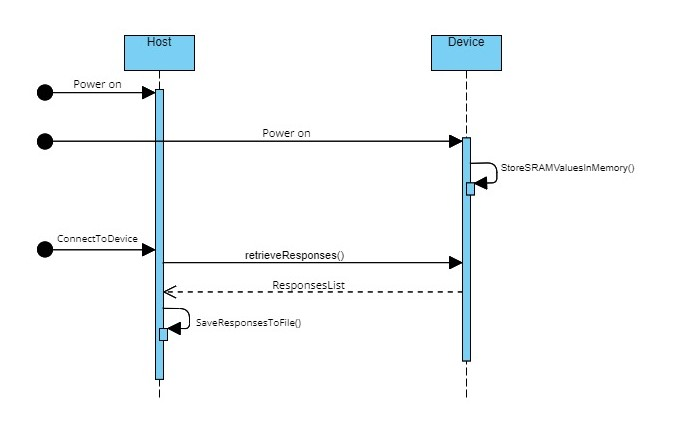
\includegraphics{images/Flow1.jpg}
  \caption{Flow 1}
  \label{fig:Flow1}
\end{figure}

\begin{figure}[H]
\centering
  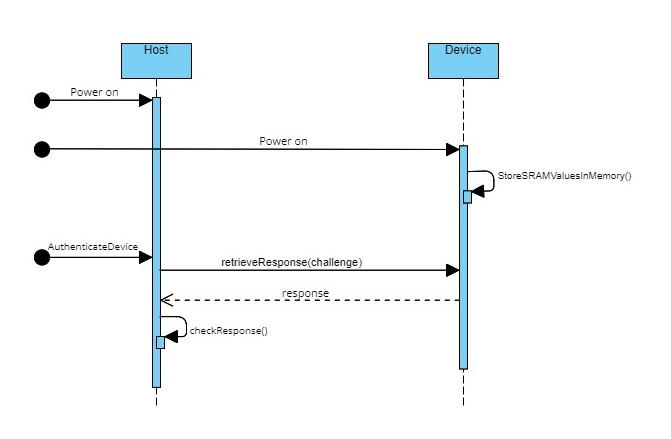
\includegraphics{images/Flow2.jpg}
  \caption{Flow 2}
  \label{fig:Flow2}
\end{figure}



%In this chapter you should provide a general overview of the project, explaining what you have implemented staying at a high-level of abstraction, without going too much into the details. Leave details for the implementation chapter. This chapter can be organized in sections, such as goal of the project, issues to be solved, solution overview, etc.\\It is very important to add images, schemes, graphs to explain the original problem and your solution. Pictures are extremely useful to understand complex ideas that might need an entire page to be explained.\\Use multiple sections to explain the starting point of your project, the last section is going to be the high-level view of your solution...so take the reader in a short `journey` to showcase your work.
